  %Thedore Ian Martiny
%Summer 2016 Test 1 Review

\documentclass[addpoints]{exam}
\newcommand{\naturals}{\mathbb{N}}
\newcommand{\integers}{\mathbb{Z}}
\newcommand{\reals}{\mathbb{R}}
\renewcommand{\baselinestretch}{1.5}
%\setlength{\textwidth}{16cm}
\usepackage{amsfonts}
\usepackage{amsmath}
\usepackage{amsthm}
\usepackage{amssymb}
\usepackage{color}
\usepackage{colortbl}
\usepackage{fullpage}
\usepackage{graphicx}
\usepackage[utf8]{inputenc}
\usepackage{listings}
\usepackage{multicol}
\usepackage{setspace}
\usepackage{wasysym}
\usepackage{xcolor}
 
\definecolor{codegreen}{rgb}{0,0.6,0}
\definecolor{codegray}{rgb}{0.5,0.5,0.5}
\definecolor{codepurple}{rgb}{0.58,0,0.82}
\definecolor{backcolour}{rgb}{0.95,0.95,0.92}
\definecolor{Gray}{gray}{0.85}
 
\lstdefinestyle{mystyle}{
    backgroundcolor=\color{backcolour},   
    commentstyle=\color{codegreen},
    keywordstyle=\color{magenta},
    numberstyle=\tiny\color{codegray},
    stringstyle=\color{codepurple},
    basicstyle=\footnotesize,
    breakatwhitespace=false,         
    breaklines=true,                 
    captionpos=b,                    
    keepspaces=true,                 
    numbers=left,                    
    numbersep=5pt,                  
    showspaces=false,                
    showstringspaces=false,
    showtabs=false,                  
    tabsize=2
}
\newcolumntype{a}{>{\columncolor{Gray}}c} 
\lstset{style=mystyle}
\begin{document}
\singlespacing

\begin{center}
  {\large\textbf{CSCI 2824 - Discrete Structures}}

  {\large\textbf{Test 1 Review}}
\end{center}

\begin{questions}
  \question Let the $U = \{1,2,3,\dots, 10\}$ be a universal set and $A =
  \{1,4,7,10\}$, $B = \{1,2,3,4,5\}$ and $C = \{2,4,6,8\}$. List the elements
  of each following set:
  \begin{parts}
    \part $\overline{A}$
    \begin{solution}
      $\overline{A} = \{2,3,5,6,8,9\}$
    \end{solution}

    \part $B \cap C$
    \begin{solution}
      $B \cap C = \{2,4\}$
    \end{solution}

    \part $\overline{B} \cap (C \backslash A)$
    \begin{solution}
      First $\overline{B} = \{6,7,8,9,10\}$ and $C\backslash A = \{2,6,8\}$.
      Thus $\overline{B} \cap (C \backslash A) = \{6,8\}$
    \end{solution}

    \part $(A\cup B) \backslash (C \backslash B)$
    \begin{solution}
      First $A\cup B = \{1,2,3,4,5,7,10\}$ and $C\backslash B = \{6,8\}$. Thus
      $(A\cup B) \backslash (C \backslash B) = \{1,2,3,4,5,7,10\}$
    \end{solution}
  \end{parts}

  \question Determine the cardinality of the following sets:

  \begin{parts}
    \part $\emptyset$
    \begin{solution}
      This is a homework 3 question.
    \end{solution}

    \part $\{\emptyset\}$
    \begin{solution}
      1
    \end{solution}

    \part $\{a,bc,d\}$
    \begin{solution}
      3
    \end{solution}

    \part $\{a,bc,d, \{a,bc,d\}\}$
    \begin{solution}
      4
    \end{solution}
  \end{parts}

  \question For the following questions determine if $A\subseteq B$ or not.
  \begin{parts}
    \part $A = \{1,2\}$, $B = \{3,2,1\}$
    \begin{solution}
      Yes.
    \end{solution}

    \part $A = \{1,2\}$, $B = \{x : x^3 - 6x^2 + 11x = 6\}$
    \begin{solution}
      Yes, the roots of $x^3-6x^2+11x=6$ are $x = 1,2,3$.
    \end{solution}

    \part $A = \{x: x^3 - 2x^2 - x + 2 = 0\}$, $B = \{x^3 - 6x^2 + 11x -6 = 0\}$
    \begin{solution}
      No, $-1 \in A$ since $-1 - 2 + 1 + 2 = 0$ but $-1\not\in B$ since $-1 - 6
      + 11 - 6 = -2$.
    \end{solution}

    \part $A = \{1,2,3,4\}$, $C = \{5,6,7,8\}$, $B = \{n : n\in A \text{ and } n
    + m = 8 \text{ for some } m\in C\}$
    \begin{solution}
      We compute $B = \{1,2,3\}$. Thus $A\not\subseteq B$.
    \end{solution}
  \end{parts}

  \question For the following questions represent the following proposition
  symbolically using the following symbols:
  \begin{center}
    p: There is a hurricane

    q: It is raining
  \end{center}

  \begin{parts}
    \part There is no hurricane
    \begin{solution}
      $\neg p$.
    \end{solution}

    \part There is a hurricane, but it is not raining.
    \begin{solution}
      $p \wedge \neg q$.
    \end{solution}

    \part Either there is a hurricane or it is raining but there is no hurricane.
    \begin{solution}
      $p \vee q \wedge \neg p$
    \end{solution}
  \end{parts}

  \question Determine the truth value of the following propositions:

  \begin{parts}
    \part If $3+5<2$ then $1+3=5$
    \begin{solution}
      True, $3+5 > 2$ so the proposition is vacuously true.
    \end{solution}

    \part $3+5 > 2$ if and only if $1 + 3 = 4$.
    \begin{solution}
      True, $3+5 >2$ and $1+3 = 4$ are both true statements thus they have the
      same truth values.
    \end{solution}
  \end{parts}

  \question Using the following statements write the following propositions in
  symbols:
  \begin{center}
    p: You run 10 laps daily

    q: You are healthy

    r: You take multi-vitamins
  \end{center}

  \begin{parts}
    \part If you run 10 laps daily, then you will be healthy.
    \begin{solution}
      $p \to q$.
    \end{solution}

    \part Taking multi-vitamins is sufficient for being healthy
    \begin{solution}
      $r \to q$.
    \end{solution}

    \part If you are healthy, then you run 10 laps daily or you do not take multi-vitamins.
    \begin{solution}
      $q \to (p \vee \neg r)$.
    \end{solution}
  \end{parts}

  \question Given that $P(x)$ denotes ``$x$ is an accountant'' and $Q(x)$
  denotes ``$x$ owns a Porsche'' write each statement symbolically.
  \begin{parts}
    \part All accountants own Porsches
    \begin{solution}
      $\forall x\, P(x) \to Q(x)$
    \end{solution}

    \part Some accountant owns a Porsche
    \begin{solution}
      $\exists x\, P(x) \wedge Q(x)$.
    \end{solution}

    \part Someone who owns a Porsche is an accountant.
    \begin{solution}
      $\exists x\, Q(x) \wedge P(x)$.
    \end{solution}
  \end{parts}

  \question Let $T(x,y)$ stand for the propositional function $x$ is taller than
  or the same height as $y$. Write all of the following propositions as words:

  \begin{parts}
    \part $\forall x\, \forall y\, T(x,y)$
    \begin{solution}
      For every pair of people $x$ and $y$, $x$ is taller or the same height as $y$.
    \end{solution}

    \part $\forall x\, \exists y\, T(x,y)$
    \begin{solution}
      For every person $x$ there is a person $y$ such that $x$ is taller than or
      the same height as $y$.
    \end{solution}

    \part $\exists x\, \exists y\, T(x,y)$
    \begin{solution}
      There is a person $x$ and a person $y$ such that $x$ is taller than or the
      same height as $y$.
    \end{solution}

    \part $\exists x\, \forall y\, T(x,y)$
    \begin{solution}
      There is a person $x$ such that for every other person $y$, $x$ is taller
      than or the same height as $y$.
    \end{solution}
  \end{parts}

  \question Prove the following claim, or provide counter examples:
  \begin{parts}
    \part For all integers $m$ and $n$, if $m$ and $m+n$ are even then $n$ is
    even.
    \begin{solution}
      This is true, if $m$ is even then $m = 2k$ for some integer $k$, if $m+n$
      is even then $m+n = 2l$ for some integer $l$. In particular:
      \begin{align*}
        m+n &= 2l\\
        2k + n &= 2l\\
        n &= 2l - 2k\\
        n &= 2(l-k)
      \end{align*}
      $l-k$ is an integer so $n$ is even.

      \qed
    \end{solution}

    \part For sets $X$, $Y$, and $Z$, if $X\subseteq Y$ then $Z\backslash Y
    \subseteq Z \backslash X$.
    \begin{solution}
      This is true, since $X$ is a ``smaller'' set we are subtracting less. Proof:

      Choose $a \in Z\backslash Y$, this tells us that $a \in Z$ and $a\not\in
      Y$. Since $X\subseteq Y$ we cannot have $a\in X$ either thus $a \in Z
      \backslash X$.

      \qed
    \end{solution}

    \part For sets $X$, $Y$, and $Z$, $X\times (Y \backslash Z) = (X \backslash
    Y) \times (X\backslash Z)$.
    \begin{solution}
      This is not true. Choose $X = \{1,2,3,4\}$, $Y = \{3,4\}$ and $Z =
      \{1,2\}$. Then $(3,3)\in X\times (Y \backslash Z)$ but $(3,3)\not\in (X
      \backslash Y) \times (X\backslash Z)$ since $3\not\in X\backslash Y$.

      \qed
    \end{solution}

    \part $\forall x\, \in \reals$ if $x^2$ is irrational then $x$ is irrational.
    \begin{solution}
      We prove this via contrapositive. If $x$ is rational then $x^2$ is
      rational. If $x$ is rational then $x = \frac{p}{q}$ then $x^2 =
      \frac{p^2}{q^2}$ which is rational. This proves the original claim.

      \qed
    \end{solution}

    \part $\sqrt[3]{2}$ is irrational.
    \begin{solution}
      This is proved the same way as that $\sqrt{2}$ is irrational:

      Proof by contradiction, suppose that $\sqrt[3]{2}$ is rational then
      $\sqrt[3]{2} = \frac{p}{q}$ where $p$ and $q$ share no common factors.
      Cubing both sides we have that $2 = \frac{p^3}{q^3}$ This means that $p^3
      = 2q^3$ which gives that $p^3$ is even. By previous results in class we
      know this means that $p$ is even as well. Thus $p = 2k$ for some integer
      $k$ or $p^3 = 8k^3$. Subbing into our above equality: $8k^3 = 2q^3$
      meaning that $q^3 = 4k^3$ meaning that $q^3$ and thus $q$ is even also.
      But then $p$ and $q$ share a factor of $2$ which is against our
      assumptions. This is our contradiction so the original claim is true.
      
      \qed
    \end{solution}

    \part For all $x,y\in \reals$ if $x$ is rational and $y$ is irrational then
    $xy$ is irrational.
    \begin{solution}
      This is not true, $x= 0$ gives that $xy = 0$ which is rational.

      \qed
    \end{solution}

    \part $(X\backslash Y) \cap (Y \backslash X) = \emptyset$ for all set $X$
    and $Y$.
    \begin{solution}
      This is true. If $a \in X \backslash Y$ then $a\in X$ but not in $Y$. If
      $b \in Y \backslash X$ then $b \in Y$ but not in $X$. To prove this is
      true we use proof by contradiction. Suppose $a\in (X\backslash Y) \cap (Y
      \backslash X)$ then $a \in X$ and not in $Y$ (from the first part of our
      intersection) but the second part tells us that $a\in Y$ and not in $X$ a
      contradiction. Thus the original claim is true.

      \qed
    \end{solution}

    \part Let $s_1,s_2, \dots,s_n$ be any real numbers. We define the average of
    these numbers as:
    \[
      A = \frac{s_1+s_2+\dots+s_n}{n}
    \]
    Suppose there exists an $i$ and a $j$ such that $s_i\not= s_j$ then there
    must be some $k$ such that $s_k > A$.
    \begin{solution}
      Proof by contradiction. Suppose that if $s_1,s_2,\dots,s_n$ are any real
      numbers and there is some $i$ and some $j$ such that $s_i\not= s_j$ but
      there is no $s_k > A$. Then either $s_i \not= A$ or $s_j \not=A$, without
      loss of generality assume that $s_i \not= A$. Then either $s_i > A$ or
      $s_i <A$. If $s_i >A$ then we are done if not then $s_i < A$ and by our
      assumption $s_k < A$ for all $k$ meaning:

      \[
        s_1 + s_2 + \dots + s_n < nA
      \]
      which contradicts $A$ being our average. Thus it must be that some $k$ has
      $s_k > A$.

      \qed
    \end{solution}

    \part For all sets $A$, $B$, and $C$, $A\subseteq C$ and $B\subseteq C$ if
    and only if $A\cup B \subseteq C$.
    \begin{solution}
      This is true. If $A\subseteq C$ and $B \subseteq C$ then for all $a\in A$,
      $a\in C$ and for all $b\in B$, $b\in C$. Thus for all $d\in A\cup B$
      either $d\in A$ (meaning $d\in C$) or $d\in B$ (meaning $d\in C$). So we
      have $A\cup B \subseteq C$.

      For the reverse if $A\cup B\subseteq C$ then this means for all $d\in
      A\cup B$, $d\in C$. Then for all $a\in A$, $a\in A\cup B$ so $a\in C$ so
      that $A\subseteq C$. Similarly for all $b\in B$, $b\in A\cup B$ so that
      $b\in C$ so $B\subseteq C.$

      \qed
    \end{solution}

    \part For all positive integers $n$ the following holds:
    \[
      \frac{1}{2n} \leq \frac{1\cdot 3 \cdot 5 \cdots (2n-1)}{2\cdot 4\cdot
      6\cdots (2n)}
    \]
    \begin{solution}
      Proof by induction. Base case $n = 1$, $\frac{1}{2} \leq \frac{1}{2}$.

      IH: For $n$ we have $\frac{1}{2n} \leq \frac{1\cdot 3\cdot 5 \cdots
      2n+1}{2\cdot 4 \cdot 6 \cdots (2n)}$.

      We show that the inequality holds for $n+1$:
      \begin{align*}
        \frac{1}{2n+2} &\leq \frac{1}{2n+2} \cdot \frac{2n+1}{2n}\\
        \intertext{This is because $2n+1 > 2n$ so the fraction is greater than 1}
        &= \frac{1}{2n}\cdot \frac{2n+1}{2n+2}\\
        \intertext{Just rearranging the fractions\dots}
        &\leq \frac{1\cdot 3\cdot 5 \cdots (2n-1)}{2\cdot 4 \cdot 6 \cdots (2n)}
          \cdot \frac{2n+1}{2n+2}\\
        \intertext{By IH\dots}
        &= \frac{1\cdot 3 \cdot 5 \cdots (2n-1)\cdot (2n+1)}{2\cdot 4\cdot 6 
          \cdots (2n)\cdot (2n+2)}
      \end{align*}

      This closes the induction.

      \qed
    \end{solution}

    \part If $X_1, X_2, \dots, X_n$ and $X$ are sets then:
    \[
      X \cap \left( X_1 \cup X_2 \cup \dots\cup X_n \right) = \left( X \cap X_1
        \right) \cup \left( X\cap X_2 \right)\cup \dots\cup \left( X\cap X_n
        \right)
    \]
    \begin{solution}
      We prove this by induction. Base case $n=1$ then the equality holds trivially.

      IH: Assume true for $n$ that is $X \cap \left( X_1 \cup X_2 \cup \dots\cup
      X_n \right) = \left( X \cap X_1 \right) \cup \left( X\cap X_2 \right)\cup
      \dots\cup \left( X\cap X_n \right)$ then we show true for $n+1$:

      \begin{align*}
        X \cap \left( X_1 \cup X_2 \cup \dots\cup X_n \cup X_{n+1}\right) &= X
          \cap \left( \left( X_1 \cup X_2 \cup \dots\cup X_n \right) \cup X_{n+1}
          \right)\\
        \intertext{Let $X_1\cup X_2 \cup \dots\cup X_n = S$, and remember our
          induction hypothesis holds true for any sets}
        &= X \cap \left( S \cup X_{n+1} \right)\\
        \intertext{Then our induction hypothesis gives:}
        &= \left( X\cap S \right) \cup \left( X \cap X_{n+1} \right)\\
        \intertext{Expanding $S$:}
        &= \left( X \cap \left( X_1 \cup X_2 \cup \dots \cup X_n \right) \right)
          \cup \left( X \cap X_{n+1} \right)\\
        \intertext{Again our IH:}
        &= \left( X \cap X_1 \right) \cup \left( X\cap X_2 \right)\cup \dots\cup
          \left( X\cap X_n \right) \cup \left( X \cap X_{n+1} \right)
      \end{align*}

      This closes the induction. 

      \qed
    \end{solution}

    \part If $X_1, X_2, \dots, X_n$ and $X$ are sets then:
    \[
      \overline{X_1\cap X_2 \cap \dots \cap X_n} = \overline{X_1} \cup
        \overline{X_2} \cup \dots \cup \overline{X_n}
    \]
    \begin{solution}
      Proof by induction. Base case, $n=1$ this is trivially true.

      IH: Assume true for $n$ that is assume $\overline{X_1\cap X_2 \cap \dots
      \cap X_n} = \overline{X_1} \cup \overline{X_2} \cup \dots \cup
      \overline{X_n}$ then we show this holds for $n+1$:

      \begin{align*}
        \overline{X_1\cap X_2 \cap \dots \cap X_n \cap X_{n+1}} &= \overline{A
          \cap X_{n+1}}\\
        \intertext{Where we let $A = X_1 \cap X_2 \cap \dots \cap X_n$, now
          using our induction hypothesis (which holds for any sets)}
        &= \overline{A} \cup \overline{X_{n+1}}\\
        \intertext{Expanding $A$:}
        &= \overline{X_1\cap X_2 \cap \dots \cap X_n} \cup \overline{X_{n+1}}\\
        \intertext{Using our induction hypothesis again:}
        &= \overline{X_1} \cup \overline{X_2} \cup \dots \cup \overline{X_n}
          \cup \overline{X_{n+1}}
      \end{align*}

      This closes the induction.

      \qed
    \end{solution}
  \end{parts}

  \question Let $f$ and $g$ be functions from the positive integers to the
  positive integers defined by
  \[
    f(n) = 2n+1, \hspace{1cm} g(n) = 3n-1
  \]
  Find the compositions $f\circ f$, $g\circ g$, $f\circ g$ and $g\circ f$.
  \begin{solution}
    \begin{align*}
      f\circ f(n) &= f(f(n))\\
      &= f(2n+1)\\
      &= 2(2n+1) + 1\\
      &= 4n + 3
    \end{align*}

    \begin{align*}
      g\circ g(n) &= g(g(n))\\
      &= g(3n-1)\\
      &= 3(3n-1) - 1\\
      &= 9n - 4
    \end{align*}

    \begin{align*}
      f\circ g(n) &= f(g(n))\\
      &= f(3n-1)\\
      &= 2(3n-1) + 1\\
      &= 6n- 1
    \end{align*}

    \begin{align*}
      g\circ f(n) &= g(f(n))\\
      &= g(2n+1)\\
      &= 3(2n+1) - 1\\
      &= 6n + 2
    \end{align*}
  \end{solution}

  \question Each of the following functions is one-to-one and thus is a
  bijective function from its domain to its image. Find the inverse of the
  given functions.
  \begin{parts}
    \part $f(x) = 4x+2$, $x\in \reals$.
    \begin{solution}
      $f^{-1}(x) = \frac{x-2}{4}$
    \end{solution}

    \part $f(x) = 3\log_2(x)$, $x\in \reals^{>0}$.
    \begin{solution}
      $f^{-1}(x) = 2^{\frac{x}{3}}$
    \end{solution}

    \part $f(x) = 6 + 2^{7x -1}$, $x\in \reals$.
    \begin{solution}
      $f^{-1}(x) = \frac{\log_2(x-6) + 1 }{7}$
    \end{solution}
  \end{parts}

  \question Let $f$ be the function from $X= \{0,1,2,3,4,5\}$ to $X$ defined by 
  \[
    f(x) = 4x\mod 6
  \]
  Write $f$ as a set of ordered pairs and draw the arrow diagram for $f$. Is $f$
  injective? Surjective?
  \begin{solution}
    $f = \{(0,0), (1,4), (2,2), (3,0), (4,4), (5,2)\}$ 

    The arrow diagram for this is:
    \begin{center}
      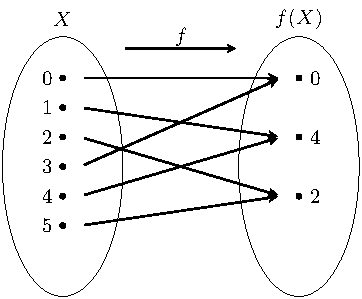
\includegraphics{arrowDiagram}
    \end{center}

    This function is not injective, both $0$ and $3$ map to $0$. This is not
    surjective since $3$ is not hit by any input.
  \end{solution}

  \question For the following questions let $g$ be a function from $X$ to $Y$
  and let $f$ be a function from $Y$ to $Z$. For each of the following if the
  statement is true prove it otherwise proved a counterexample.
  \begin{parts}
    \part If $g$ is onto then $f\circ g$ is onto.
    \begin{solution}
      This is not true, let $X = Y = Z = \{1,2,3\}$ define $f(x) = 1 $ for all
      $x\in Y$ and let $g(x) = x$ for all $x\in X$. Then $g$ is onto, but $f$ is
      not. Then $f\circ g$ is not onto because there is no input which will map
      to $2$ (all inputs eventually go to Rome\dots I mean 1).
    \end{solution}

    \part If $f\circ g$ is injective then $f$ is injective.
    \begin{solution}
      This is not true. Consider $Y = Z = \{1,2,3\}$ and $X = \{ 1,2\}$ and let
      $f(1) = 1, f(2) =1,$ and $f(3) = 2$. $f$ is clearly not injective. Define
      $g(1) = 2$ and $g(2) =3$. $g$ clearly is injective. Then we have that no
      two inputs to $f\circ g$ map to the same output, so that $f\circ g$ is
      injective, but $f$ is not.
    \end{solution}

    \part If $f$ is one-to-one then $f\circ g$ is one-to-one.
    \begin{solution}
      Again not true. Let $X = Y = Z = \{1,2,3\}$ and define $f(x) = x$ for all
      $x\in Y$ then $f$ is one-to-one. Define $g(1) = 1, g(2) = 1$, and $g(3) =
      2$. $f\circ g (1) = 1$ and $f\circ g(2) = 1$ meaning that $f\circ g$ is
      not one-to-one.
    \end{solution}
  \end{parts}
\end{questions}
\end{document}
